\documentclass[a4paper]{article}
\usepackage[utf8]{inputenc}
\usepackage{fullpage}
\usepackage{amsmath,amssymb}
\usepackage[colorlinks]{hyperref} % use colored text in stead of ugly boxes
\usepackage[toc]{multitoc} % Nice two-column TOC

%~ \usepackage{enumerate} 
\usepackage{pgf}
\usepackage{tikz}
\usepackage{pictures/tikz-uml}

%~ \usepackage{listings}
%~ \lstset{language=java, tabsize=4, frame=single,basicstyle=\scriptsize}

\title{Programming Life - Requirements Analysis and Design }

\author{Group 5/E:\\
Felix Akkermans \\
Niels Doekemeijer \\
Thomas van Helden \\
Albert ten Napel \\
Jan Pieter Waagmeester}

\begin{document}
\maketitle
\begin{center}

\end{center}

%
\vfill

\small{\tableofcontents}
\pagebreak
\section{Introduction} 		% (Niels)
The purpose of biotechnology is to use micro-organisms like moulds and bacteria for the production of chemical substances. These chemical substances are used as energy (biofuels), in products (bioplastics), in food and in medicine. Not only can these micro-organisms produce, they can also be used to break down chemical substances, for example in the purification of water.\footnote{Programming Life – Contextproject assignment (Dick de Ridder, Marcel Reinders)}

Using molecular biology, these micro-organisms can be altered to add, change or remove functionality. This is done by mutating the DNA of the organism. Synthetic biology is the science in which biology and engineering are combined to create new biological functionality\footnote{Programming Life – Contextproject kickoff (Dick de Ridder, Marcel Reinders)}. The engineering part is made easier by using biobricks\footnote{\url{http://biobricks.org/}}. These “bricks” are simple genetic circuits which provide a basic functionality (for example the imitation of an OR or AND gate) and share a common interface. By combining these biobricks, a new biological systems can be engineered.

In its abstract form, this system can be visualized as a logical circuit, but in the organism the circuit corresponds with a group of molecules (proteins, genes, RNA) that react with each other. How (and if) they will react depends on many different elements, like the concentration and reaction speed of a protein. This reaction can be simulated using a (heavily) simplified model.\footnote{see footnote 1}

In this report, we will describe the design of a visual modeling environment for synthetic biology, in which biotechnologists can design, simulate and validate a logical circuit built using biobricks. We will clarify our proposed system using a list of requirements (2.1), a few analysis models (2.4), a business object model (2.5), a few dynamic models (2.6) and a preliminary drawing of the interface (2.7). In chapter 3 we will give a planning of the following of the project.

\section{Proposed system}
\subsection{Overview} 		% (Niels)
In this document, we will provide an analysis and design proposal for a visual modeling environment for synthetic biology, in which biotechnologists can design, simulate and validate a logical circuit built using biobricks.

\subsection{Functional requirements} % (Felix en Thomas)
\subsection{Nonfunctional requirements and constraints} % (Felix en Thomas)
\subsection{Analysis models}
\subsubsection{Use case model, descriptions and scenarios}
\begin{figure}[h!]
	\caption{Use cases}
	\begin{center}
	%simple use case, depending on tikz-uml
\begin{tikzpicture}
\begin{umlsystem}[x=4.5, y=4, fill=red!10]{Biobrick modeller/simulator}
        \umlusecase[y=-0.5, x=-1.5]{Start application}
        \umlusecase[y=-5.5, x=4]{Model Biobrick}
        \umlusecase[y=-8, x=4]{Simulate}
        \umlusecase[y=-3.5, x=4]{Export SBML}
        \umlusecase[y=-1.5, x=4]{Import SBML}
        
        \umlusecase[y=-7, x=10]{Specify protein}
        \umlusecase[y=-3, x=10]{View available proteins}
        
        \umlusecase[y=-9, x=0]{Quit application}
\end{umlsystem}

\umlactor{user}

\umlassoc{user}{usecase-1}
\umlassoc{user}{usecase-2}
\umlassoc{user}{usecase-3}
\umlassoc{user}{usecase-4}
\umlassoc{user}{usecase-5}
\umlassoc{user}{usecase-8}
\umlinclude{usecase-2}{usecase-6}
\umlinclude{usecase-2}{usecase-1}
\umlinclude{usecase-3}{usecase-1}
\umlinclude{usecase-4}{usecase-1}
\umlinclude{usecase-5}{usecase-1}
\umlextend{usecase-2}{usecase-3}
\umlextend{usecase-2}{usecase-7}

\end{tikzpicture}

	\end{center}
\end{figure}
\subsection{Business Object model} % (Albert)
\begin{figure}[h!]
	\caption{Business Object model}
	\begin{center}
		% documentation on tikz-uml:
% http://www.ensta-paristech.fr/~kielbasi/tikzuml/index.php?lang=en&id=doc#t-1.1
\begin{tikzpicture}

\umlclass{Protein}{
  concentration \\
  $K_m$ \\
  $n$ \\
}{}
\umlclass[y=-6]{BioBrick}{
  proteins \\
  gates \\
}{}
\umlclass[x=6,y=-6]{Circuit}{bricks[]}{}

\umlclass[x=6,y=0]{SBML}{circuit}{}



\umlassoc[mult1=*, mult2=*]{Protein}{BioBrick}
\umlassoc[mult1=*, mult2=*]{Circuit}{BioBrick}
\umlinherit[geometry=-|, arg1=represents,align1=right]{SBML}{Circuit}
\end{tikzpicture}


	\end{center}
\end{figure}

\subsection{Dynamic models}
\subsection{Interface} % (Jan Pieter)
\begin{figure}[h!]
	\caption{Quick mockup of the Graphical user interface}
	\begin{center}
	%~ 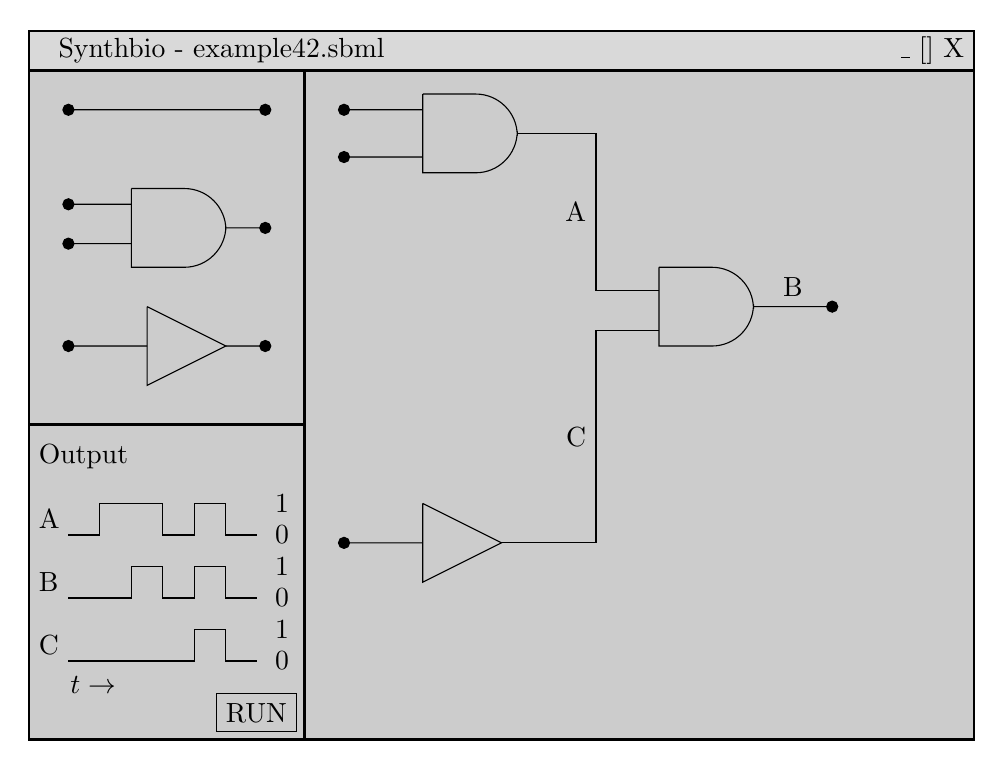
\begin{tikzpicture}

%main window
\draw[fill=black!20,line width=1] (-6,4) rectangle (6, -5);

% window title bar
\draw[fill=black!15,line width=1] (-6,4) rectangle (6, 3.5);
\node [anchor=west] at (-5.75, 3.75) {Synthbio - example42.sbml};
\node [anchor=east] at (6, 3.75) {\_ [] X};

% sidebar
\draw[fill=black!20,line width=1] (-6, 3.5) rectangle (-2.5, -5);
\draw[line width=1] (-6, -1) -- (-2.5, -1);

% wire
\draw (-5.5, 3) [fill]circle (2pt) -- ++( 2.5, 0) circle (2pt);

%and
\draw (-4.7, 2) [rounded corners=15pt] --  ++(1.2, 0)  -- ++(0, -1) [sharp corners] -- ++(-1.2, 0) -- ++(0, 1);
\filldraw (-5.5, 1.8) circle (2pt) -- (-4.7, 1.8);
\filldraw (-5.5, 1.3) circle (2pt) -- (-4.7, 1.3);
\filldraw (-3.5, 1.5) -- (-3, 1.5) circle (2pt);

%not
\draw (-4.5, 0.5) --  ++(1, -0.5) -- ++(-1, -.5) -- ++(0, 1);
\draw (-5.5, 0) [fill] circle (2pt) -- ++(1,0);
\draw (-3.5, 0) -- ++(.5, 0) [fill] circle (2pt);

%output
\node [anchor=west] at ( -6, -1.4) {Output};
\node [anchor=west] at(-5.6, -4.3) {$t \to$};

%signal A
\node [anchor=west] at ( -6, -2.2) {A};
\node [anchor=west] at ( -3, -2) {1};
\node [anchor=west] at ( -3, -2.4) {0};
\draw (-5.5, -2.4) -- ++(.4, 0) -- ++(0, .4) -- ++ (0.8, 0) -- ++(0, -.4) -- ++(.4, 0) -- ++(0, .4) -- ++(.4, 0) -- ++(0, -.4) -- ++(.4, 0);

%signal B
\node [anchor=west] at ( -6, -3) {B};
\node [anchor=west] at ( -3, -2.8) {1};
\node [anchor=west] at ( -3, -3.2) {0};
\draw (-5.5, -3.2) -- ++(.8, 0) -- ++(0, .4) -- ++ (0.4, 0) -- ++(0, -.4) -- ++(.4, 0) -- ++(0, .4) -- ++(.4, 0) -- ++(0, -.4) -- ++(.4, 0);

%signal C
\node [anchor=west] at ( -6, -3.8) {C};
\node [anchor=west] at ( -3, -3.6) {1};
\node [anchor=west] at ( -3, -4) {0};
\draw (-5.5, -4) -- ++(1.6, 0) -- ++(0, .4) -- ++ (0.4, 0) -- ++(0, -.4) --  ++(.4, 0);

%run button
\node [draw, anchor=south east] at (-2.6, -4.9) {RUN};

% Working area

%and gate
\draw (-2, 3) [fill]circle (2pt) -- ++(1, 0);
\draw (-2, 2.4) [fill]circle (2pt) -- ++(1, 0);
\draw (-1, 3.2) [rounded corners=15pt] --  ++(1.2, 0)  -- ++(0, -1) [sharp corners] -- ++(-1.2, 0) -- ++(0, 1);

%signal B
\draw (0.2, 2.7) -- ++ (1, 0) -- node[left] {A} ++(0, -2) -- ++(.8, 0);

%another gate
\draw (2, 1) [rounded corners=15pt] --  ++(1.2, 0)  -- ++(0, -1) [sharp corners] -- ++(-1.2, 0) -- ++(0, 1);

\draw (3.2, .5) -- node[above] {B} ++(1, 0) [fill] circle (2pt);

%not gate
\draw (-2, -2.5) [fill]circle (2pt) --  ++(1, 0);
\draw (-1, -2) --  ++(1, -0.5) -- ++(-1, -.5) -- ++(0, 1);

% signal C
\draw (0, -2.5) -- ++(1.2, 0) -- node[left] {C} ++(0, 2.7) -- ++ (.8, 0);

\end{tikzpicture}

	\end{center}
\end{figure}

\section{Planning}  % (Felix)
\section{Glossary} % (Jan Pieter)
\begin{description}
	\item[Bio brick] blah
	\item[DNA] \text{Deoxyribonucleic acid} is a very long molecule containing the information needed to support the life in allmost all creatures.
	\item[Protein] is a complex molecule
	\item[RNA] Working copy of the
	\item[SBML] \textit{Systems Biology Markup Language} is a XML-based format for storage of various computermodels of biological processes.
\end{description}
\end{document}